%%%%%%%%%%%%%%%%%%%%%%%%%%%%%%%%%%%%%%%%%%%%%%%%%%%%%%%%%%%%%%%%%%%%
%% I, the copyright holder of this work, release this work into the
%% public domain. This applies worldwide. In some countries this may
%% not be legally possible; if so: I grant anyone the right to use
%% this work for any purpose, without any conditions, unless such
%% conditions are required by law.
%%%%%%%%%%%%%%%%%%%%%%%%%%%%%%%%%%%%%%%%%%%%%%%%%%%%%%%%%%%%%%%%%%%%

\documentclass{beamer}
\usetheme[logopath=./, logo=fig/logo-tu.png]{fibeamer}
\usepackage[utf8]{inputenc}
\usepackage[
  main=english, %% By using `czech` or `slovak` as the main locale
                %% instead of `english`, you can typeset the
                %% presentation in either Czech or Slovak,
                %% respectively.
  czech, slovak %% The additional keys allow foreign texts to be
]{babel}        %% typeset as follows:
%%
%%   \begin{otherlanguage}{czech}   ... \end{otherlanguage}
%%   \begin{otherlanguage}{slovak}  ... \end{otherlanguage}
%%
%% These macros specify information about the presentation
\title{Robust Gate Detection for Autonomous Drone Racing} %% that will be typeset on the
\subtitle{Mid-Term Presentation} %% title page.
\author{Philipp Dürnay\\ \bigskip \bigskip Guido de Chroon \hfill	
\includegraphics[width=3cm]{fig/mavlab}\\
	 David M. J. Tax  \hfill 
\includegraphics[width=3cm]{fig/prgroup}%
}
%% These additional packages are used within the document:
\usepackage{ragged2e}  % `\justifying` text
\usepackage{booktabs}  % Tables
\usepackage{tabularx}
\usepackage{tikz}      % Diagrams
\usetikzlibrary{calc, shapes, backgrounds}
\usepackage{amsmath, amssymb}
\usepackage{url}       % `\url`s
\usepackage{listings}  % Code listings
\frenchspacing
\begin{document}
  \frame{\maketitle}

  %\AtBeginSection[2,3,4]{% Print an outline at the beginning of sections
  %  \begin{frame}<beamer>
  %    \frametitle{Outline for Section \thesection}
  %    \tableofcontents[currentsection]
  %  \end{frame}}

  \begin{darkframes}
  	\begin{frame}{Outline}
  		\tableofcontents
  	\end{frame}
	\section{Introduction}
	\subsection{Application}
    \begin{frame}{IROS2018}
    	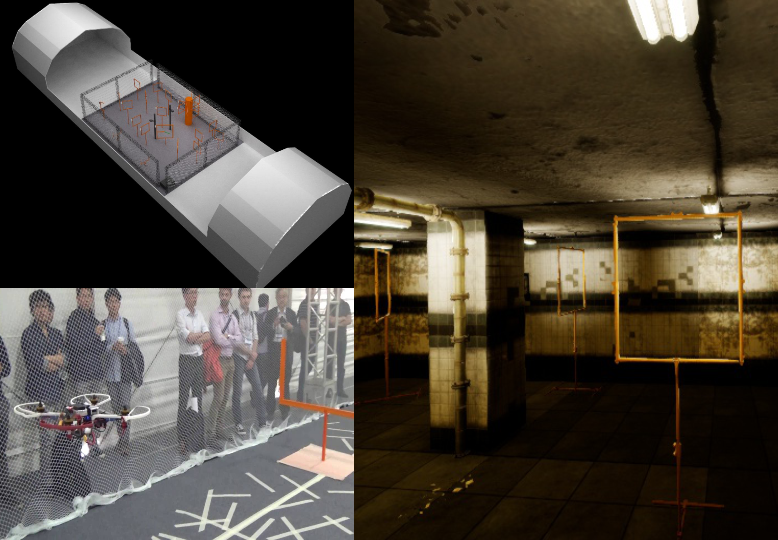
\includegraphics[width=\textwidth]{fig/application}
    \end{frame}
    \begin{frame}{Current Method}
       	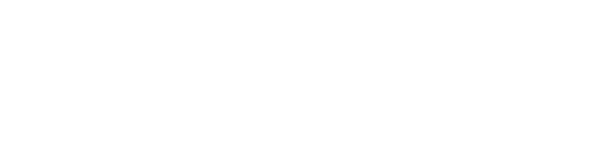
\includegraphics[width=\textwidth]{fig/current_method}
    \end{frame}

	\subsection{Research Problem}    
	\begin{frame}{Research Problem}
	\textbf{Efficient and robust detection of wire frame objects with limited resources.}
	\end{frame}
    
    \section{Background}
    \begin{frame}{Outline for Section \thesection}
    \tableofcontents[currentsection]
	\end{frame}
\subsection{Object Detection}
	\begin{frame}{Object Detection}
	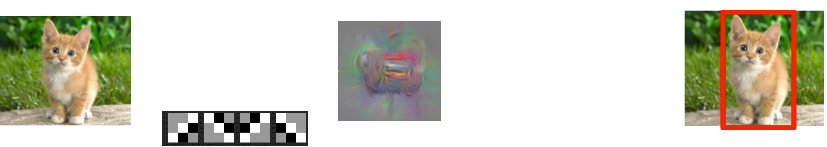
\includegraphics[width=\textwidth]{fig/ObjectDetection}
	\end{frame}
% if you look at object detection on a high level basis, you basically see this pipeline
% You have your input image and at the end you want to have a bounding box that tells you which object is where in the image for example with such a bounding box,
% so usually you preprocess the image by extracting certain features from the image
% so you have filters that look for certain colours or an eye or an ear for example,
% this gives you an internal representation of the image with the important aspects
% then you do two tasks and that is classification and localization so determining the object and the bounding box coordinates
% Now there are different ways for each of these steps but thats it from a high level perspective
% State of the art methods all use convolutional neural networks and the reason that is beliefed to be responsible for that performance is the fact that you can combine all these steps in one model and train it end to end on the task so instead of manually enginnering and training models you combine it all in one.
	\subsection{Convolutional Neural Networks}
		\begin{frame}{Convolutional Networks}
	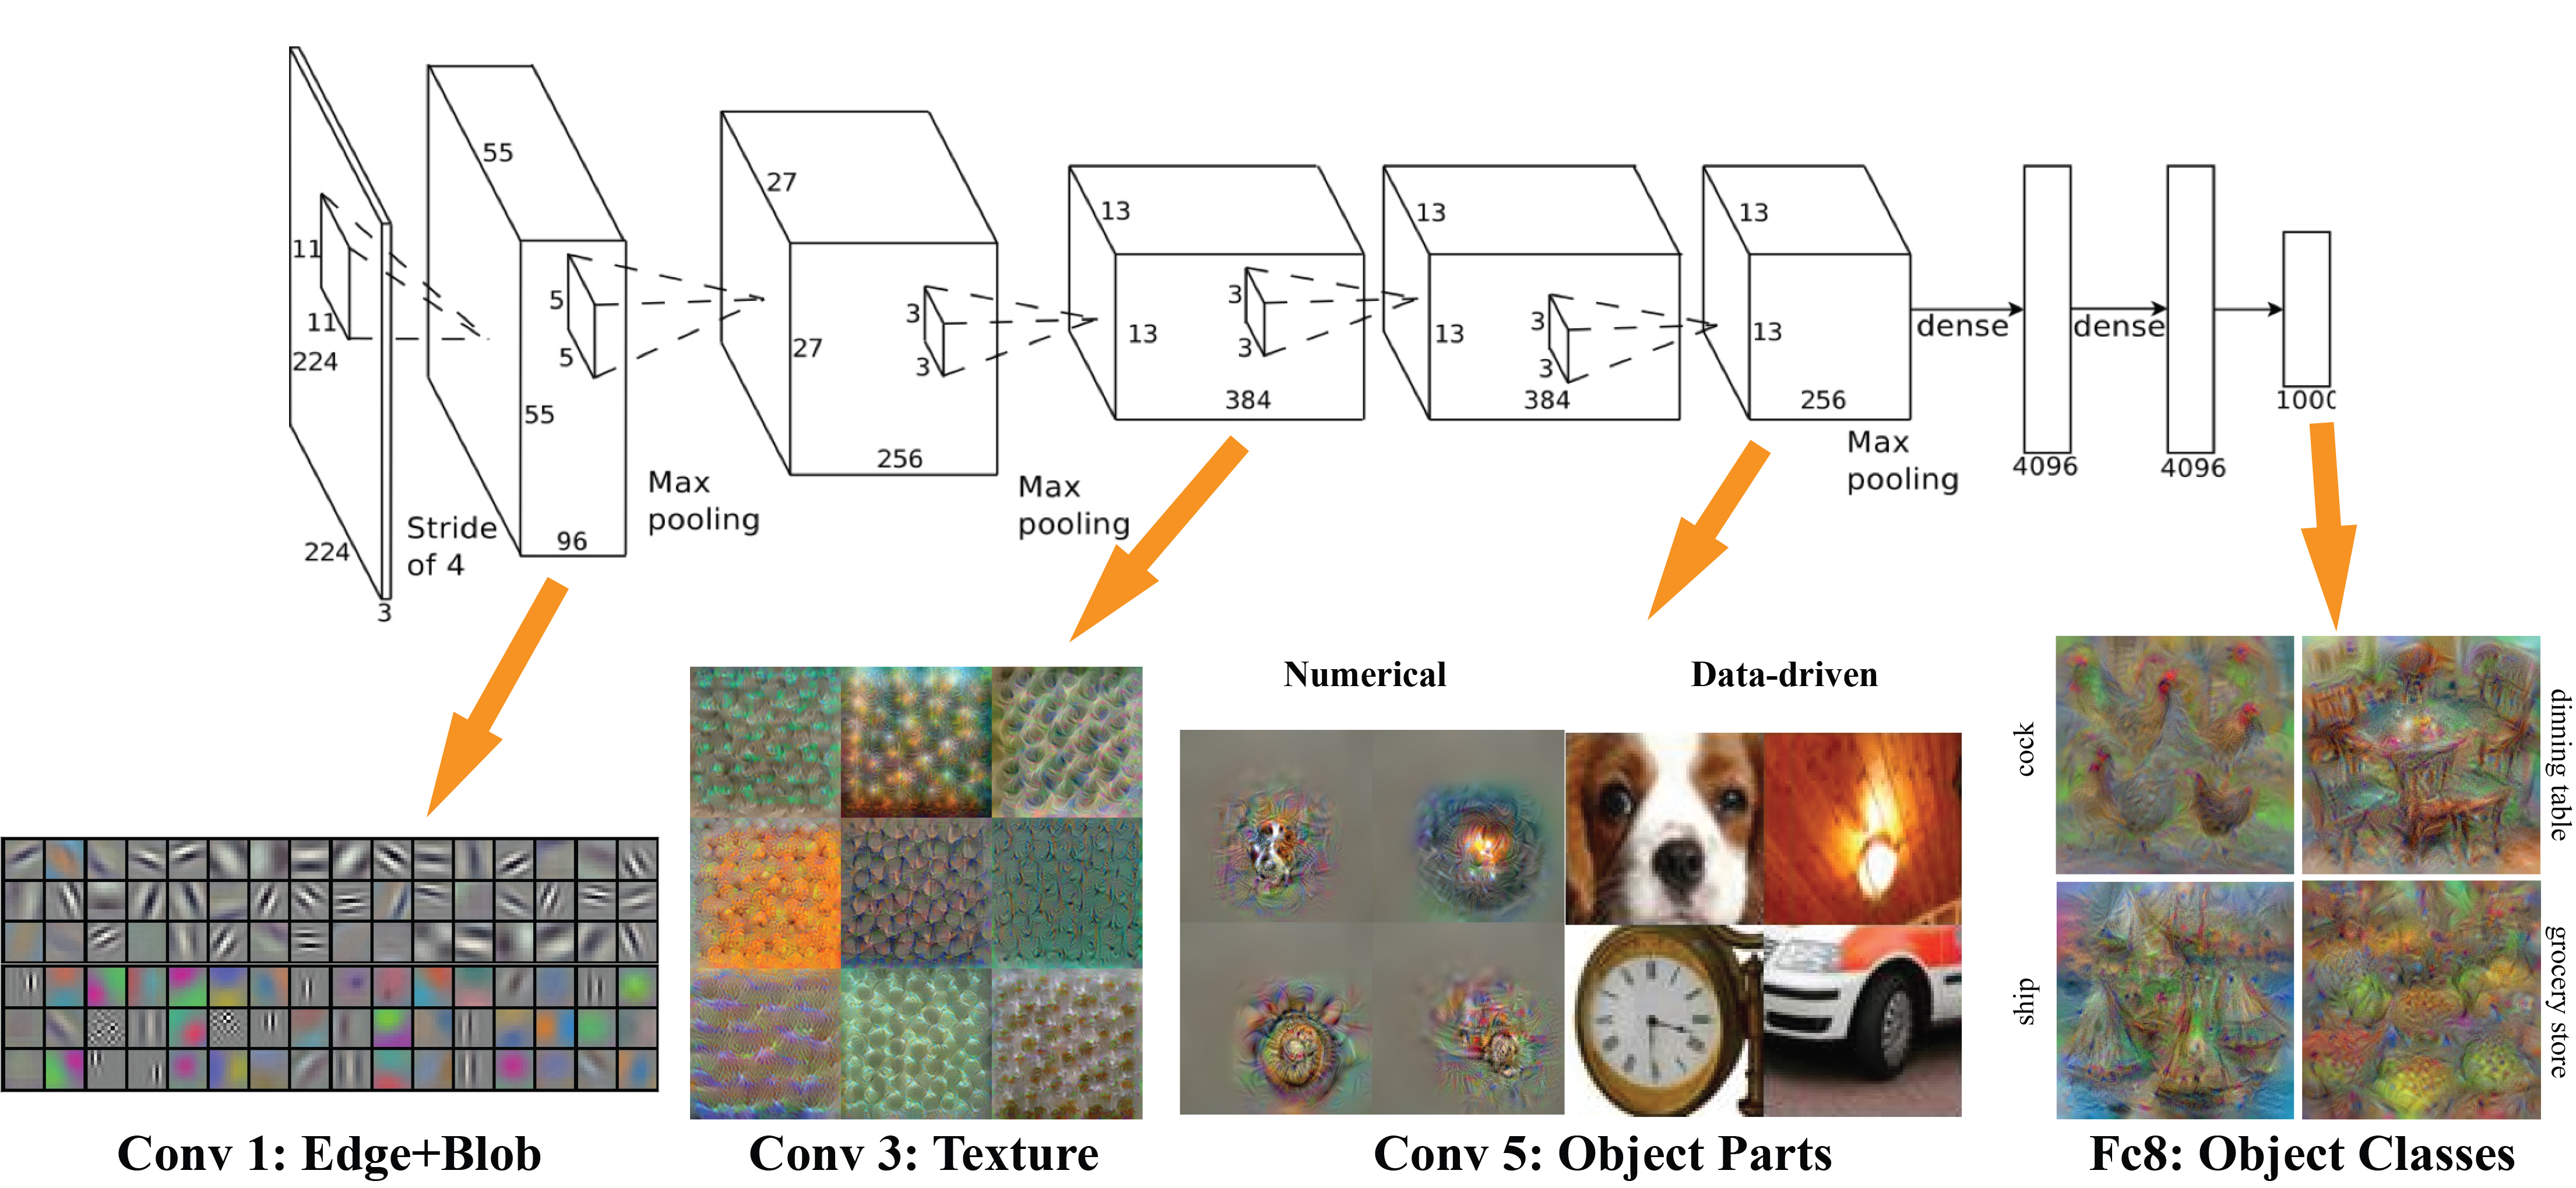
\includegraphics[width=\textwidth]{fig/cnn}
\end{frame}

% So now we can look at an example for a convolutional network and at the different layers. So typically you apply per layer a certain amount of filters, then you apply pooling and non-linearity and you stack several of these filters and at the end you have your output.
% And typically the performance improves the deeper you go. One reason is that the flexibility of the model increases but you can also look at it from another perspective and see what the different layers are responsible for. So when you visualize these filters you usually see how these early layers look for edges, corner and blobs, while higher layers then combine these low level features to more complex parts like eyes, noses and so on.
% Now the draw back of these deep networks is their computational effort, especially the deep one is their huge consumption in energy, computations and memory which makes them not applicable for micro air vehicles.
% But if we now rethink to the objects we want to detect so wire frame objects, racing gates that mostly consist of edges and corners, these final layers should not be very useful. So a much smaller model should actually be sufficient. 
    \section{Approach}
        \begin{frame}{Outline for Section \thesection}
    \tableofcontents[currentsection]
\end{frame}
  \subsection{Method}
    \begin{frame}{Approach}
  Hypothesis: A much smaller network should be able to learn the task.
  TODO drawing
    \end{frame}
    
    \subsection{Results}
    \begin{frame}{Results}
    	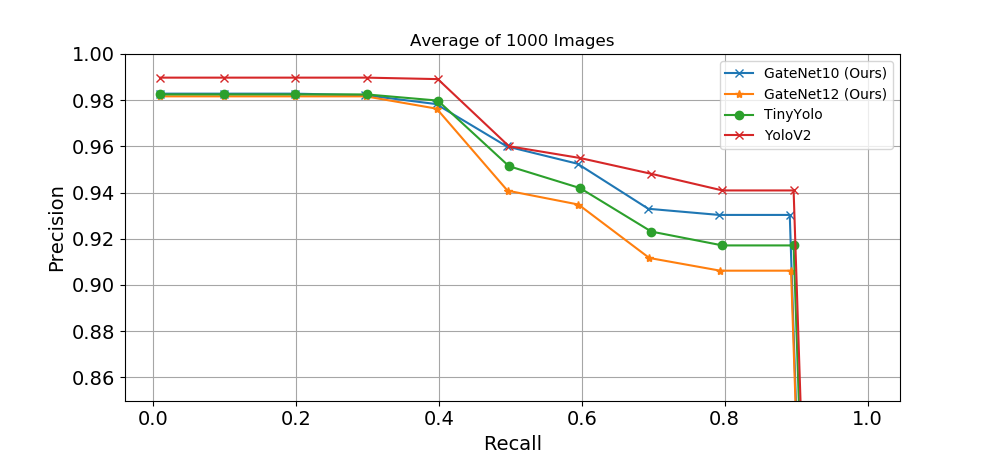
\includegraphics[width=\textwidth]{fig/pr}
    \end{frame}

    \begin{frame}{Results - Examples}
    	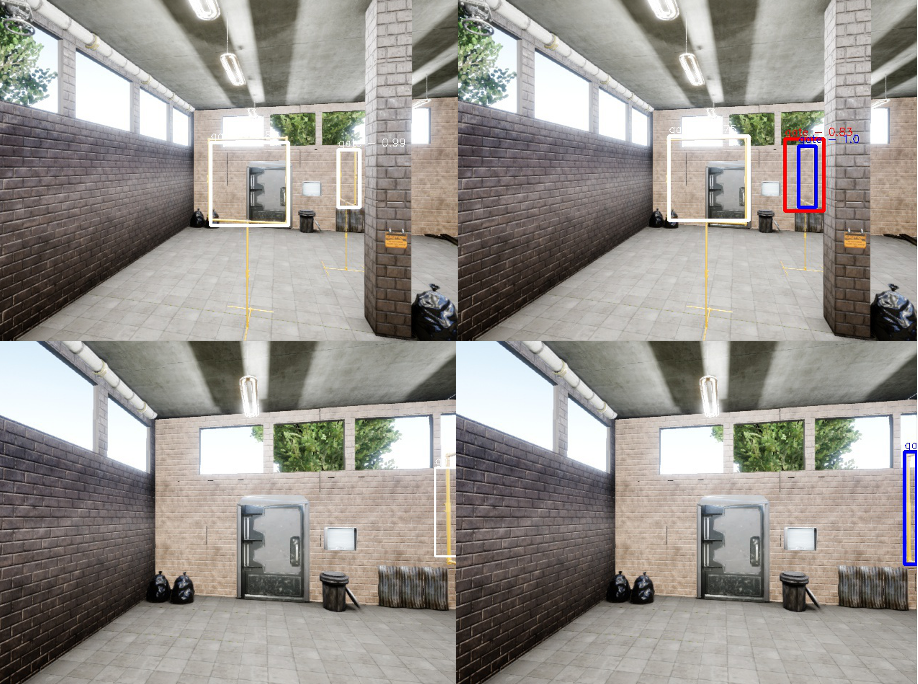
\includegraphics[width=\textwidth]{fig/examples}
	\end{frame}
    
    \section{Conclusion}
    \begin{frame}{Conclusion}

    \begin{itemize}
    	\item Initial assumption confirmed. Much less layers are necessary. However, 9 layers is still quite deep.
    	\item Deeper layers don't serve much but objects in difficult poses are detected better.
    	\item Number of filters can largely be reduced.
    	\item Reduction in parameters does not lead to same equal reduction in speedup.
    \end{itemize}
    \end{frame}

    \begin{frame}{Next Steps}
    	\begin{itemize}
    		\item Analyzing what the deeper layers learn.
    		\item Investigating speed bottlenecks.
    		\item Investigating further methods to reduce model size/ speed up computations.
    	\end{itemize}
    \end{frame}
    

    \begin{frame}{Questions}
    \centering
\huge ?
    	\end{frame}
    
    
  \end{darkframes}

\end{document}
